\documentclass{article}

\usepackage{amsmath}
\usepackage{palatino}
\usepackage{tikz}

\newcommand{\carrier}[1]{|#1|}
\newcommand{\ar}[1]{\mathbf{ar(#1)}}
\newcommand{\kcat}{\mathbf{K}}
\newcommand{\facat}{\textbf{F-Alg}}

\begin{document}
\begin{enumerate}
\item [2.2.1]
  We want to show that the definition of a homomorphism in an $\Omega$-algebra is equivalent to the definition of a homomorphism in an $F$-algebra with signature $\Omega$.
  
  \subitem 
  First, let $\ar{\omega}$ denote the arity of each operator symbol $\omega \in \Omega$.
  Additionally let $a_\omega$ be the interpretation of the operator symbol $a$ in the $\Omega$-algebra $A$.
  A homomorphism between $\Omega$-algebras $A$ and $B$ is a function $h : \carrier{A} \rightarrow \carrier{B}$ such that for each $\omega \in \Omega$ and $(x_1,\ldots,x_{\ar{\omega}}) \in \carrier{A}^{\ar{\omega}}$,
  \begin{align}
    h(a_\omega~(x_1,\ldots,x_{\ar{\omega}})) = b_\omega~(h(x_1),\ldots,h(x_{\ar{\omega}}))
  \end{align}

  \subitem 
  Next, an $F$-homomorphism is defined as a function $h : \carrier{A} \rightarrow\carrier{B}$ making the following diagram commute.
  \begin{center}
    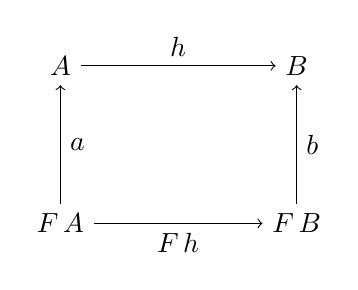
\begin{tikzpicture}
      \node (1) {$A$};
      \node[right of=1,xshift=2cm] (2) {$B$};
      \node[below of=1,yshift=-1cm] (3) {$F\,A$};
      \node[right of=3,xshift=2cm] (4) {$F\,B$};

      \draw[->] (1) -- node[above] {$h$} (2);
      \draw[->] (3) -- node[right] {$a$} (1);
      \draw[->] (3) -- node[below]{$F\,h$} (4);
      \draw[->] (4) -- node[right] {$b$} (2);
    \end{tikzpicture}
  \end{center}

  \subitem 
  To prove equivalence, we first show that if $h$ is an $\Omega$-homomorphism then the diagram must commute.
  This follows immediately from the definition of an $\Omega$-homomorphism; the composition $h \circ a$ applied to the object $(\omega, (x_1,\ldots,x_{\ar{\omega}})) \in F\,A$ is exactly $h(a_\omega, (x_1,\ldots,x_{\ar{\omega}}))$.
  We know by definition that this is equivalent to $b_\omega~(h(x_1),\ldots,h(x_{\ar{\omega}}))$, which is exactly the composition $b \circ F\,h$ applied to the object $(\omega, (x_1,\ldots,x_{\ar{\omega}})) \in F\,B$.

  \subitem 
  Conversely, if the diagram commutes then $h$ must be an $\Omega$-homomorphism because the compositions $h \circ a$ and $b \circ F\,h$ are equal.
  Thus the equation (1) proving that $h$ is an $\Omega$-homomorphism holds.

\newpage
\item [2.2.4.1]
  If $\kcat$ is a category and $F: \kcat \rightarrow \kcat$ is an endofunctor on $\kcat$ then the $F$-algebras and $F$-homomorphisms over $\kcat$ form a category $\facat$ as follows:
  \begin{itemize}
  \item Objects are $F$-algebras.
  \item Morphisms are $F$-homomorphisms.
  \item Identities are lifted from $\kcat$.
  \subitem If $id_A : A \rightarrow A$ is the identity on an object $A \in \kcat$ then we get a morphism $F\,id_A : F\,A \rightarrow F\,A$ because $id_A$ is trivially a structure-preserving map (homomorphism) between objects in $\kcat$ and therefore $F$ must have an arrow $F\,id_A$ making the analog of the above diagram commute.
  \item Composition is similarly lifted from $\kcat$.
  \subitem If there exist homomorphisms $h_{AB} : A \rightarrow B$ and $h_{BC} : B \rightarrow C$ then the composition $h_{BC} \circ h_{AB}$ must exist in the category $\kcat$.
    This composition is also trivially a homomorphism $h_{AC}$ from $A$ to $B$ and therefore the arrow $F\,h_{AC} = F\,h_{BC} \circ F\,h_{AB}$ must exist in the category $\facat$.
  \end{itemize}

\newpage
\item [2.2.4.2]
  The goal is to show that if an $F$-algebra $(A,a)$ is initial in the category $\facat$ then $a$ is an isomorphism.

  \subitem 
  Consider the $\kcat$-object $F\,A$.
  We know it exists because $F : \kcat \rightarrow \kcat$ must be defined on all objects $A \in \kcat$.
  Furthermore, we know it must be the carrier of some object $F\,F\,A$ because the pair $(F\,A, F\,a)$ form an $F$-algebra.
  Moreover, the initiality of $F\,A$ uniquely determines an arrow $F\,h : F\,A \rightarrow F\,F\,A$.
  Thus the $h$ in $F\,h$ must be an arrow $h : A \rightarrow F\,A$.
  In particular, it must be the inverse of $a : F\,A \rightarrow A$.
  
  \subitem 
  Pictorally, we have the following diagram where $F\,h$ is determined by the initiality of $F\,A$ and $h$ follows as a consequence:
  \begin{center}
    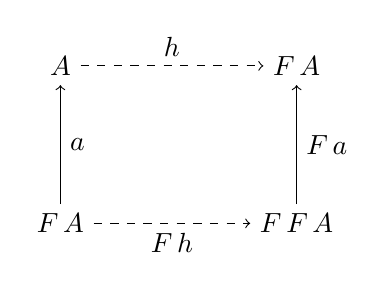
\begin{tikzpicture}
      \node (1) {$A$};
      \node[right of=1,xshift=2cm] (2) {$F\,A$};
      \node[below of=1,yshift=-1cm] (3) {$F\,A$};
      \node[right of=3,xshift=2cm] (4) {$F\,F\,A$};

      \draw[dashed,->] (1) -- node[above] {$h$} (2);
      \draw[->] (3) -- node[right] {$a$} (1);
      \draw[dashed,->] (3) -- node[below]{$F\,h$} (4);
      \draw[->] (4) -- node[right] {$F\,a$} (2);
    \end{tikzpicture}
  \end{center}

  \subitem 
  This initial object $(A,a)$ corresponds to a fixed point of $F$ because there is an isomorphism between $F\,A$ and $A$ and similarly between $F\,a$ and $a$.
  
\end{enumerate}
\end{document}

